\documentclass[a4paper]{book}
\usepackage{a4wide}
\usepackage{makeidx}
\usepackage{graphicx}
\usepackage{multicol}
\usepackage{float}
\usepackage{listings}
\usepackage{color}
\usepackage{textcomp}
\usepackage{alltt}
\usepackage{times}
\usepackage{ifpdf}
\ifpdf
\usepackage[pdftex,
            pagebackref=true,
            colorlinks=true,
            linkcolor=blue,
            unicode
           ]{hyperref}
\else
\usepackage[ps2pdf,
            pagebackref=true,
            colorlinks=true,
            linkcolor=blue,
            unicode
           ]{hyperref}
\usepackage{pspicture}
\fi
\usepackage[utf8]{inputenc}
\usepackage{doxygen}
\lstset{language=C++,inputencoding=utf8,basicstyle=\footnotesize,breaklines=true,breakatwhitespace=true,tabsize=8,numbers=left }
\makeindex
\setcounter{tocdepth}{3}
\renewcommand{\footrulewidth}{0.4pt}
\begin{document}
\hypersetup{pageanchor=false}
\begin{titlepage}
\vspace*{7cm}
\begin{center}
{\Large RLEG \\[1ex]\large 1 }\\
\vspace*{1cm}
{\large Generated by Doxygen 1.6.3}\\
\vspace*{0.5cm}
{\small Thu Jun 6 20:09:26 2013}\\
\end{center}
\end{titlepage}
\clearemptydoublepage
\pagenumbering{roman}
\tableofcontents
\clearemptydoublepage
\pagenumbering{arabic}
\hypersetup{pageanchor=true}
\chapter{Data Structure Index}
\section{Data Structures}
Here are the data structures with brief descriptions\-:\begin{DoxyCompactList}
\item\contentsline{section}{\hyperlink{structIMU__DATA__STRUCT_1_1calibrated}{I\-M\-U\-\_\-\-D\-A\-T\-A\-\_\-\-S\-T\-R\-U\-C\-T\-::calibrated} }{\pageref{structIMU__DATA__STRUCT_1_1calibrated}}{}
\item\contentsline{section}{\hyperlink{classCartesian__controller}{Cartesian\-\_\-controller} }{\pageref{classCartesian__controller}}{}
\item\contentsline{section}{\hyperlink{classCartesian__pose__controller}{Cartesian\-\_\-pose\-\_\-controller} }{\pageref{classCartesian__pose__controller}}{}
\item\contentsline{section}{\hyperlink{classCartesian__velocity__controller}{Cartesian\-\_\-velocity\-\_\-controller} }{\pageref{classCartesian__velocity__controller}}{}
\item\contentsline{section}{\hyperlink{structDATA__XYZ}{D\-A\-T\-A\-\_\-\-X\-Y\-Z} \\*A structure to represent a 3d Vector }{\pageref{structDATA__XYZ}}{}
\item\contentsline{section}{\hyperlink{structDATA__XYZ__DOUBLE}{D\-A\-T\-A\-\_\-\-X\-Y\-Z\-\_\-\-D\-O\-U\-B\-L\-E} \\*Vector definition on double }{\pageref{structDATA__XYZ__DOUBLE}}{}
\item\contentsline{section}{\hyperlink{structDQ}{D\-Q} \\*Dual\-Quaternion library Header }{\pageref{structDQ}}{}
\item\contentsline{section}{\hyperlink{structDUMMY__MATRICES}{D\-U\-M\-M\-Y\-\_\-\-M\-A\-T\-R\-I\-C\-E\-S} }{\pageref{structDUMMY__MATRICES}}{}
\item\contentsline{section}{\hyperlink{structEFF__DATA__STRUCT}{E\-F\-F\-\_\-\-D\-A\-T\-A\-\_\-\-S\-T\-R\-U\-C\-T} }{\pageref{structEFF__DATA__STRUCT}}{}
\item\contentsline{section}{\hyperlink{structGDATALOGGER}{G\-D\-A\-T\-A\-L\-O\-G\-G\-E\-R} }{\pageref{structGDATALOGGER}}{}
\item\contentsline{section}{\hyperlink{structGDATALOGGERIPC__SHM}{G\-D\-A\-T\-A\-L\-O\-G\-G\-E\-R\-I\-P\-C\-\_\-\-S\-H\-M} }{\pageref{structGDATALOGGERIPC__SHM}}{}
\item\contentsline{section}{\hyperlink{structGDATALOGGERVARIABLE}{G\-D\-A\-T\-A\-L\-O\-G\-G\-E\-R\-V\-A\-R\-I\-A\-B\-L\-E} }{\pageref{structGDATALOGGERVARIABLE}}{}
\item\contentsline{section}{\hyperlink{structGMATLABDATAFILECONFIG}{G\-M\-A\-T\-L\-A\-B\-D\-A\-T\-A\-F\-I\-L\-E\-C\-O\-N\-F\-I\-G} }{\pageref{structGMATLABDATAFILECONFIG}}{}
\item\contentsline{section}{\hyperlink{structGMATRIX}{G\-M\-A\-T\-R\-I\-X} }{\pageref{structGMATRIX}}{}
\item\contentsline{section}{\hyperlink{structGMATRIX__MATLAB__DATAHEAD}{G\-M\-A\-T\-R\-I\-X\-\_\-\-M\-A\-T\-L\-A\-B\-\_\-\-D\-A\-T\-A\-H\-E\-A\-D} }{\pageref{structGMATRIX__MATLAB__DATAHEAD}}{}
\item\contentsline{section}{\hyperlink{structGQUEUECONTROL}{G\-Q\-U\-E\-U\-E\-C\-O\-N\-T\-R\-O\-L} }{\pageref{structGQUEUECONTROL}}{}
\item\contentsline{section}{\hyperlink{structIMU__DATA__STRUCT}{I\-M\-U\-\_\-\-D\-A\-T\-A\-\_\-\-S\-T\-R\-U\-C\-T} \\*Data of I\-M\-U structure }{\pageref{structIMU__DATA__STRUCT}}{}
\item\contentsline{section}{\hyperlink{structIMU__PARAM__STRUCT}{I\-M\-U\-\_\-\-P\-A\-R\-A\-M\-\_\-\-S\-T\-R\-U\-C\-T} \\*Configs of I\-M\-U }{\pageref{structIMU__PARAM__STRUCT}}{}
\item\contentsline{section}{\hyperlink{structLink}{Link} }{\pageref{structLink}}{}
\item\contentsline{section}{\hyperlink{structMATLAB__DATAHEAD}{M\-A\-T\-L\-A\-B\-\_\-\-D\-A\-T\-A\-H\-E\-A\-D} }{\pageref{structMATLAB__DATAHEAD}}{}
\item\contentsline{section}{\hyperlink{classMatrix}{Matrix} }{\pageref{classMatrix}}{}
\item\contentsline{section}{\hyperlink{structMRA__DATA__STRUCT}{M\-R\-A\-\_\-\-D\-A\-T\-A\-\_\-\-S\-T\-R\-U\-C\-T} \\*Struct to control M\-R\-A }{\pageref{structMRA__DATA__STRUCT}}{}
\item\contentsline{section}{\hyperlink{structIMU__PARAM__STRUCT_1_1param__acc}{I\-M\-U\-\_\-\-P\-A\-R\-A\-M\-\_\-\-S\-T\-R\-U\-C\-T\-::param\-\_\-acc} \\*Accelerometer Parameters }{\pageref{structIMU__PARAM__STRUCT_1_1param__acc}}{}
\item\contentsline{section}{\hyperlink{structIMU__PARAM__STRUCT_1_1param__gyr}{I\-M\-U\-\_\-\-P\-A\-R\-A\-M\-\_\-\-S\-T\-R\-U\-C\-T\-::param\-\_\-gyr} \\*Gyrometer Parameters }{\pageref{structIMU__PARAM__STRUCT_1_1param__gyr}}{}
\item\contentsline{section}{\hyperlink{structIMU__PARAM__STRUCT_1_1param__mag}{I\-M\-U\-\_\-\-P\-A\-R\-A\-M\-\_\-\-S\-T\-R\-U\-C\-T\-::param\-\_\-mag} \\*Magnetometer Parameters }{\pageref{structIMU__PARAM__STRUCT_1_1param__mag}}{}
\item\contentsline{section}{\hyperlink{structQ}{Q} }{\pageref{structQ}}{}
\item\contentsline{section}{\hyperlink{structRobot}{Robot} \\*The Structure holding the relevant info of a \hyperlink{structRobot}{Robot} }{\pageref{structRobot}}{}
\item\contentsline{section}{\hyperlink{structSPI__PARAM__STRUCT}{S\-P\-I\-\_\-\-P\-A\-R\-A\-M\-\_\-\-S\-T\-R\-U\-C\-T} \\*Configs for S\-P\-I }{\pageref{structSPI__PARAM__STRUCT}}{}
\end{DoxyCompactList}

\chapter{Data Structure Documentation}
\hypertarget{structIMU__DATA__STRUCT_1_1calibrated}{\section{I\-M\-U\-\_\-\-D\-A\-T\-A\-\_\-\-S\-T\-R\-U\-C\-T\-:\-:calibrated Struct Reference}
\label{structIMU__DATA__STRUCT_1_1calibrated}\index{I\-M\-U\-\_\-\-D\-A\-T\-A\-\_\-\-S\-T\-R\-U\-C\-T\-::calibrated@{I\-M\-U\-\_\-\-D\-A\-T\-A\-\_\-\-S\-T\-R\-U\-C\-T\-::calibrated}}
}


{\ttfamily \#include \char`\"{}communication.\-h\char`\"{}}



Collaboration diagram for I\-M\-U\-\_\-\-D\-A\-T\-A\-\_\-\-S\-T\-R\-U\-C\-T\-:\-:calibrated\-:\nopagebreak
\begin{figure}[H]
\begin{center}
\leavevmode
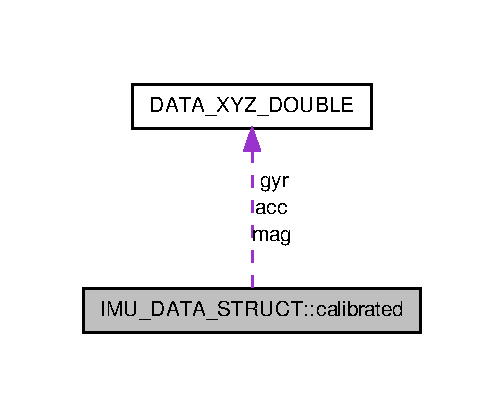
\includegraphics[width=242pt]{structIMU__DATA__STRUCT_1_1calibrated__coll__graph}
\end{center}
\end{figure}
\subsection*{Data Fields}
\begin{DoxyCompactItemize}
\item 
\hyperlink{structDATA__XYZ__DOUBLE}{D\-A\-T\-A\-\_\-\-X\-Y\-Z\-\_\-\-D\-O\-U\-B\-L\-E} \hyperlink{structIMU__DATA__STRUCT_1_1calibrated_a281a7fdb40a05ed97388f18b9bb90c81}{acc}
\item 
\hyperlink{structDATA__XYZ__DOUBLE}{D\-A\-T\-A\-\_\-\-X\-Y\-Z\-\_\-\-D\-O\-U\-B\-L\-E} \hyperlink{structIMU__DATA__STRUCT_1_1calibrated_a8a54aded6ce608f1b7d2b4a0c52c248b}{gyr}
\item 
\hyperlink{structDATA__XYZ__DOUBLE}{D\-A\-T\-A\-\_\-\-X\-Y\-Z\-\_\-\-D\-O\-U\-B\-L\-E} \hyperlink{structIMU__DATA__STRUCT_1_1calibrated_a2fde6c6759e0fda17e272c32096cb9ec}{mag}
\end{DoxyCompactItemize}


\subsection{Detailed Description}


Definition at line 94 of file communication.\-h.



\subsection{Field Documentation}
\hypertarget{structIMU__DATA__STRUCT_1_1calibrated_a281a7fdb40a05ed97388f18b9bb90c81}{\index{I\-M\-U\-\_\-\-D\-A\-T\-A\-\_\-\-S\-T\-R\-U\-C\-T\-::calibrated@{I\-M\-U\-\_\-\-D\-A\-T\-A\-\_\-\-S\-T\-R\-U\-C\-T\-::calibrated}!acc@{acc}}
\index{acc@{acc}!IMU_DATA_STRUCT::calibrated@{I\-M\-U\-\_\-\-D\-A\-T\-A\-\_\-\-S\-T\-R\-U\-C\-T\-::calibrated}}
\subsubsection[{acc}]{\setlength{\rightskip}{0pt plus 5cm}{\bf D\-A\-T\-A\-\_\-\-X\-Y\-Z\-\_\-\-D\-O\-U\-B\-L\-E} I\-M\-U\-\_\-\-D\-A\-T\-A\-\_\-\-S\-T\-R\-U\-C\-T\-::calibrated\-::acc}}\label{structIMU__DATA__STRUCT_1_1calibrated_a281a7fdb40a05ed97388f18b9bb90c81}


Definition at line 95 of file communication.\-h.



Referenced by calibrate\-\_\-imu(), datalogger\-\_\-update(), ui\-\_\-imu\-\_\-data(), and ui\-\_\-overview\-\_\-data().

\hypertarget{structIMU__DATA__STRUCT_1_1calibrated_a8a54aded6ce608f1b7d2b4a0c52c248b}{\index{I\-M\-U\-\_\-\-D\-A\-T\-A\-\_\-\-S\-T\-R\-U\-C\-T\-::calibrated@{I\-M\-U\-\_\-\-D\-A\-T\-A\-\_\-\-S\-T\-R\-U\-C\-T\-::calibrated}!gyr@{gyr}}
\index{gyr@{gyr}!IMU_DATA_STRUCT::calibrated@{I\-M\-U\-\_\-\-D\-A\-T\-A\-\_\-\-S\-T\-R\-U\-C\-T\-::calibrated}}
\subsubsection[{gyr}]{\setlength{\rightskip}{0pt plus 5cm}{\bf D\-A\-T\-A\-\_\-\-X\-Y\-Z\-\_\-\-D\-O\-U\-B\-L\-E} I\-M\-U\-\_\-\-D\-A\-T\-A\-\_\-\-S\-T\-R\-U\-C\-T\-::calibrated\-::gyr}}\label{structIMU__DATA__STRUCT_1_1calibrated_a8a54aded6ce608f1b7d2b4a0c52c248b}


Definition at line 96 of file communication.\-h.



Referenced by calibrate\-\_\-imu(), datalogger\-\_\-update(), ui\-\_\-imu\-\_\-data(), and ui\-\_\-overview\-\_\-data().

\hypertarget{structIMU__DATA__STRUCT_1_1calibrated_a2fde6c6759e0fda17e272c32096cb9ec}{\index{I\-M\-U\-\_\-\-D\-A\-T\-A\-\_\-\-S\-T\-R\-U\-C\-T\-::calibrated@{I\-M\-U\-\_\-\-D\-A\-T\-A\-\_\-\-S\-T\-R\-U\-C\-T\-::calibrated}!mag@{mag}}
\index{mag@{mag}!IMU_DATA_STRUCT::calibrated@{I\-M\-U\-\_\-\-D\-A\-T\-A\-\_\-\-S\-T\-R\-U\-C\-T\-::calibrated}}
\subsubsection[{mag}]{\setlength{\rightskip}{0pt plus 5cm}{\bf D\-A\-T\-A\-\_\-\-X\-Y\-Z\-\_\-\-D\-O\-U\-B\-L\-E} I\-M\-U\-\_\-\-D\-A\-T\-A\-\_\-\-S\-T\-R\-U\-C\-T\-::calibrated\-::mag}}\label{structIMU__DATA__STRUCT_1_1calibrated_a2fde6c6759e0fda17e272c32096cb9ec}


Definition at line 97 of file communication.\-h.



Referenced by calibrate\-\_\-imu(), datalogger\-\_\-update(), ui\-\_\-imu\-\_\-data(), and ui\-\_\-overview\-\_\-data().



The documentation for this struct was generated from the following file\-:\begin{DoxyCompactItemize}
\item 
communication/\hyperlink{communication_2communication_8h}{communication.\-h}\end{DoxyCompactItemize}

\hypertarget{structDATA__XYZ}{
\section{DATA\_\-XYZ Struct Reference}
\label{structDATA__XYZ}\index{DATA\_\-XYZ@{DATA\_\-XYZ}}
}


A structure to represent a 3d Vector.  




{\ttfamily \#include \char`\"{}communication.h\char`\"{}}

\subsection*{Data Fields}
\begin{DoxyCompactItemize}
\item 
short int \hyperlink{structDATA__XYZ_a54c1596e9f9969fd9c21e8458024ecfb}{x}
\item 
short int \hyperlink{structDATA__XYZ_a94bbb1c889bf53eb6a5fffa2b39322cf}{y}
\item 
short int \hyperlink{structDATA__XYZ_a69e89ab0ec6e5d72fc5d54f62cc07fb5}{z}
\end{DoxyCompactItemize}


\subsection{Detailed Description}
A structure to represent a 3d Vector. 

Definition at line 75 of file communication.h.



\subsection{Field Documentation}
\hypertarget{structDATA__XYZ_a54c1596e9f9969fd9c21e8458024ecfb}{
\index{DATA\_\-XYZ@{DATA\_\-XYZ}!x@{x}}
\index{x@{x}!DATA_XYZ@{DATA\_\-XYZ}}
\subsubsection[{x}]{\setlength{\rightskip}{0pt plus 5cm}short int {\bf DATA\_\-XYZ::x}}}
\label{structDATA__XYZ_a54c1596e9f9969fd9c21e8458024ecfb}


Definition at line 76 of file communication.h.



Referenced by calibrate\_\-imu(), control\_\-main(), datalogger\_\-update(), periodic\_\-task\_\-2(), read\_\-all\_\-data(), ui\_\-eff\_\-data(), ui\_\-imu\_\-data(), and ui\_\-overview\_\-data().

\hypertarget{structDATA__XYZ_a94bbb1c889bf53eb6a5fffa2b39322cf}{
\index{DATA\_\-XYZ@{DATA\_\-XYZ}!y@{y}}
\index{y@{y}!DATA_XYZ@{DATA\_\-XYZ}}
\subsubsection[{y}]{\setlength{\rightskip}{0pt plus 5cm}short int {\bf DATA\_\-XYZ::y}}}
\label{structDATA__XYZ_a94bbb1c889bf53eb6a5fffa2b39322cf}


Definition at line 77 of file communication.h.



Referenced by calibrate\_\-imu(), datalogger\_\-update(), periodic\_\-task\_\-2(), read\_\-all\_\-data(), ui\_\-eff\_\-data(), ui\_\-imu\_\-data(), and ui\_\-overview\_\-data().

\hypertarget{structDATA__XYZ_a69e89ab0ec6e5d72fc5d54f62cc07fb5}{
\index{DATA\_\-XYZ@{DATA\_\-XYZ}!z@{z}}
\index{z@{z}!DATA_XYZ@{DATA\_\-XYZ}}
\subsubsection[{z}]{\setlength{\rightskip}{0pt plus 5cm}short int {\bf DATA\_\-XYZ::z}}}
\label{structDATA__XYZ_a69e89ab0ec6e5d72fc5d54f62cc07fb5}


Definition at line 78 of file communication.h.



Referenced by calibrate\_\-imu(), control\_\-main(), datalogger\_\-update(), periodic\_\-task\_\-2(), read\_\-all\_\-data(), ui\_\-eff\_\-data(), ui\_\-imu\_\-data(), and ui\_\-overview\_\-data().



The documentation for this struct was generated from the following file:\begin{DoxyCompactItemize}
\item 
communication/\hyperlink{communication_8h}{communication.h}\end{DoxyCompactItemize}

\hypertarget{structDATA__XYZ__DOUBLE}{
\section{DATA\_\-XYZ\_\-DOUBLE Struct Reference}
\label{structDATA__XYZ__DOUBLE}\index{DATA\_\-XYZ\_\-DOUBLE@{DATA\_\-XYZ\_\-DOUBLE}}
}


Vector definition on double.  




{\ttfamily \#include \char`\"{}communication.h\char`\"{}}

\subsection*{Data Fields}
\begin{DoxyCompactItemize}
\item 
double \hyperlink{structDATA__XYZ__DOUBLE_a22868cc99a423900e7b82d015a5eb91f}{x}
\item 
double \hyperlink{structDATA__XYZ__DOUBLE_a198a27b5df3b5b0bf461b0e481e22a82}{y}
\item 
double \hyperlink{structDATA__XYZ__DOUBLE_a9556e8868c223ff3e28756ea18a284c0}{z}
\end{DoxyCompactItemize}


\subsection{Detailed Description}
Vector definition on double. 

Definition at line 84 of file communication.h.



\subsection{Field Documentation}
\hypertarget{structDATA__XYZ__DOUBLE_a22868cc99a423900e7b82d015a5eb91f}{
\index{DATA\_\-XYZ\_\-DOUBLE@{DATA\_\-XYZ\_\-DOUBLE}!x@{x}}
\index{x@{x}!DATA_XYZ_DOUBLE@{DATA\_\-XYZ\_\-DOUBLE}}
\subsubsection[{x}]{\setlength{\rightskip}{0pt plus 5cm}double {\bf DATA\_\-XYZ\_\-DOUBLE::x}}}
\label{structDATA__XYZ__DOUBLE_a22868cc99a423900e7b82d015a5eb91f}


Definition at line 85 of file communication.h.



Referenced by calibrate\_\-imu(), datalogger\_\-update(), ui\_\-imu\_\-data(), and ui\_\-overview\_\-data().

\hypertarget{structDATA__XYZ__DOUBLE_a198a27b5df3b5b0bf461b0e481e22a82}{
\index{DATA\_\-XYZ\_\-DOUBLE@{DATA\_\-XYZ\_\-DOUBLE}!y@{y}}
\index{y@{y}!DATA_XYZ_DOUBLE@{DATA\_\-XYZ\_\-DOUBLE}}
\subsubsection[{y}]{\setlength{\rightskip}{0pt plus 5cm}double {\bf DATA\_\-XYZ\_\-DOUBLE::y}}}
\label{structDATA__XYZ__DOUBLE_a198a27b5df3b5b0bf461b0e481e22a82}


Definition at line 86 of file communication.h.



Referenced by calibrate\_\-imu(), datalogger\_\-update(), ui\_\-imu\_\-data(), and ui\_\-overview\_\-data().

\hypertarget{structDATA__XYZ__DOUBLE_a9556e8868c223ff3e28756ea18a284c0}{
\index{DATA\_\-XYZ\_\-DOUBLE@{DATA\_\-XYZ\_\-DOUBLE}!z@{z}}
\index{z@{z}!DATA_XYZ_DOUBLE@{DATA\_\-XYZ\_\-DOUBLE}}
\subsubsection[{z}]{\setlength{\rightskip}{0pt plus 5cm}double {\bf DATA\_\-XYZ\_\-DOUBLE::z}}}
\label{structDATA__XYZ__DOUBLE_a9556e8868c223ff3e28756ea18a284c0}


Definition at line 87 of file communication.h.



Referenced by calibrate\_\-imu(), datalogger\_\-update(), ui\_\-imu\_\-data(), and ui\_\-overview\_\-data().



The documentation for this struct was generated from the following file:\begin{DoxyCompactItemize}
\item 
communication/\hyperlink{communication_8h}{communication.h}\end{DoxyCompactItemize}

\hypertarget{structEFF__DATA__STRUCT}{
\section{EFF\_\-DATA\_\-STRUCT Struct Reference}
\label{structEFF__DATA__STRUCT}\index{EFF\_\-DATA\_\-STRUCT@{EFF\_\-DATA\_\-STRUCT}}
}


{\ttfamily \#include \char`\"{}communication.h\char`\"{}}



Collaboration diagram for EFF\_\-DATA\_\-STRUCT:\subsection*{Data Fields}
\begin{DoxyCompactItemize}
\item 
\hyperlink{structDATA__XYZ}{DATA\_\-XYZ} \hyperlink{structEFF__DATA__STRUCT_abe8952947b54bf9c247f3429ee3aeb44}{F}
\item 
\hyperlink{structDATA__XYZ}{DATA\_\-XYZ} \hyperlink{structEFF__DATA__STRUCT_aaf6e03b6e600295e0f5c706fc869e9d1}{M}
\item 
uint8\_\-t \hyperlink{structEFF__DATA__STRUCT_aa42ebc512dd79fa6ebf998162a149446}{new\_\-data}
\end{DoxyCompactItemize}


\subsection{Detailed Description}


Definition at line 112 of file communication.h.



\subsection{Field Documentation}
\hypertarget{structEFF__DATA__STRUCT_abe8952947b54bf9c247f3429ee3aeb44}{
\index{EFF\_\-DATA\_\-STRUCT@{EFF\_\-DATA\_\-STRUCT}!F@{F}}
\index{F@{F}!EFF_DATA_STRUCT@{EFF\_\-DATA\_\-STRUCT}}
\subsubsection[{F}]{\setlength{\rightskip}{0pt plus 5cm}{\bf DATA\_\-XYZ} {\bf EFF\_\-DATA\_\-STRUCT::F}}}
\label{structEFF__DATA__STRUCT_abe8952947b54bf9c247f3429ee3aeb44}


Definition at line 113 of file communication.h.



Referenced by datalogger\_\-update(), read\_\-all\_\-data(), and ui\_\-eff\_\-data().

\hypertarget{structEFF__DATA__STRUCT_aaf6e03b6e600295e0f5c706fc869e9d1}{
\index{EFF\_\-DATA\_\-STRUCT@{EFF\_\-DATA\_\-STRUCT}!M@{M}}
\index{M@{M}!EFF_DATA_STRUCT@{EFF\_\-DATA\_\-STRUCT}}
\subsubsection[{M}]{\setlength{\rightskip}{0pt plus 5cm}{\bf DATA\_\-XYZ} {\bf EFF\_\-DATA\_\-STRUCT::M}}}
\label{structEFF__DATA__STRUCT_aaf6e03b6e600295e0f5c706fc869e9d1}


Definition at line 114 of file communication.h.



Referenced by ui\_\-eff\_\-data().

\hypertarget{structEFF__DATA__STRUCT_aa42ebc512dd79fa6ebf998162a149446}{
\index{EFF\_\-DATA\_\-STRUCT@{EFF\_\-DATA\_\-STRUCT}!new\_\-data@{new\_\-data}}
\index{new\_\-data@{new\_\-data}!EFF_DATA_STRUCT@{EFF\_\-DATA\_\-STRUCT}}
\subsubsection[{new\_\-data}]{\setlength{\rightskip}{0pt plus 5cm}uint8\_\-t {\bf EFF\_\-DATA\_\-STRUCT::new\_\-data}}}
\label{structEFF__DATA__STRUCT_aa42ebc512dd79fa6ebf998162a149446}


Definition at line 115 of file communication.h.



Referenced by datalogger\_\-update(), and read\_\-all\_\-data().



The documentation for this struct was generated from the following file:\begin{DoxyCompactItemize}
\item 
communication/\hyperlink{communication_8h}{communication.h}\end{DoxyCompactItemize}

\hypertarget{structIMU__DATA__STRUCT}{\section{I\-M\-U\-\_\-\-D\-A\-T\-A\-\_\-\-S\-T\-R\-U\-C\-T Struct Reference}
\label{structIMU__DATA__STRUCT}\index{I\-M\-U\-\_\-\-D\-A\-T\-A\-\_\-\-S\-T\-R\-U\-C\-T@{I\-M\-U\-\_\-\-D\-A\-T\-A\-\_\-\-S\-T\-R\-U\-C\-T}}
}


Data of I\-M\-U structure.  




{\ttfamily \#include \char`\"{}communication (\-Cópia em conflito de Caio Gustavo Mesquita Angelo 2013-\/05-\/17).\-h\char`\"{}}

\subsection*{Data Structures}
\begin{DoxyCompactItemize}
\item 
struct \hyperlink{structIMU__DATA__STRUCT_1_1calibrated}{calibrated}
\end{DoxyCompactItemize}
\subsection*{Data Fields}
\begin{DoxyCompactItemize}
\item 
\hyperlink{structDATA__XYZ}{D\-A\-T\-A\-\_\-\-X\-Y\-Z} \hyperlink{structIMU__DATA__STRUCT_a448f284bf44eb503affda586ad5fa9d2}{acc}
\begin{DoxyCompactList}\small\item\em Accel Vector. \end{DoxyCompactList}\item 
\hyperlink{structDATA__XYZ}{D\-A\-T\-A\-\_\-\-X\-Y\-Z} \hyperlink{structIMU__DATA__STRUCT_a0c1ac26626e4434a2ee124a1928a23a1}{gyr}
\begin{DoxyCompactList}\small\item\em Gyrometer Vector. \end{DoxyCompactList}\item 
\hyperlink{structDATA__XYZ}{D\-A\-T\-A\-\_\-\-X\-Y\-Z} \hyperlink{structIMU__DATA__STRUCT_a40c7df8b6d49297aa52873cfd9b60daa}{mag}
\begin{DoxyCompactList}\small\item\em Magnetormeter Vector. \end{DoxyCompactList}\item 
struct \hyperlink{structIMU__DATA__STRUCT_1_1calibrated}{I\-M\-U\-\_\-\-D\-A\-T\-A\-\_\-\-S\-T\-R\-U\-C\-T\-::calibrated} \hyperlink{structIMU__DATA__STRUCT_aeffe3c3c5a7191a5cef16e7aab6c3795}{calib}
\item 
short int \hyperlink{structIMU__DATA__STRUCT_a81e1dbf765c1d947ca6076aa1bbc73e7}{temp}
\item 
double \hyperlink{structIMU__DATA__STRUCT_a3553fcee6beba17fe0c7711ac0483875}{calib\-\_\-temp}
\item 
uint8\-\_\-t \hyperlink{structIMU__DATA__STRUCT_a99924252176326418863e511d4fa437b}{new\-\_\-data}
\end{DoxyCompactItemize}


\subsection{Detailed Description}
Data of I\-M\-U structure. 

Definition at line 61 of file communication (\-Cópia em conflito de Caio Gustavo Mesquita Angelo 2013-\/05-\/17).\-h.



\subsection{Field Documentation}
\hypertarget{structIMU__DATA__STRUCT_a448f284bf44eb503affda586ad5fa9d2}{\index{I\-M\-U\-\_\-\-D\-A\-T\-A\-\_\-\-S\-T\-R\-U\-C\-T@{I\-M\-U\-\_\-\-D\-A\-T\-A\-\_\-\-S\-T\-R\-U\-C\-T}!acc@{acc}}
\index{acc@{acc}!IMU_DATA_STRUCT@{I\-M\-U\-\_\-\-D\-A\-T\-A\-\_\-\-S\-T\-R\-U\-C\-T}}
\subsubsection[{acc}]{\setlength{\rightskip}{0pt plus 5cm}{\bf D\-A\-T\-A\-\_\-\-X\-Y\-Z} I\-M\-U\-\_\-\-D\-A\-T\-A\-\_\-\-S\-T\-R\-U\-C\-T\-::acc}}\label{structIMU__DATA__STRUCT_a448f284bf44eb503affda586ad5fa9d2}


Accel Vector. 



Definition at line 62 of file communication (\-Cópia em conflito de Caio Gustavo Mesquita Angelo 2013-\/05-\/17).\-h.



Referenced by calibrate\-\_\-imu(), control\-\_\-main(), datalogger\-\_\-update(), main(), periodic\-\_\-task\-\_\-2(), read\-\_\-all\-\_\-data(), ui\-\_\-imu\-\_\-data(), and ui\-\_\-overview\-\_\-data().

\hypertarget{structIMU__DATA__STRUCT_aeffe3c3c5a7191a5cef16e7aab6c3795}{\index{I\-M\-U\-\_\-\-D\-A\-T\-A\-\_\-\-S\-T\-R\-U\-C\-T@{I\-M\-U\-\_\-\-D\-A\-T\-A\-\_\-\-S\-T\-R\-U\-C\-T}!calib@{calib}}
\index{calib@{calib}!IMU_DATA_STRUCT@{I\-M\-U\-\_\-\-D\-A\-T\-A\-\_\-\-S\-T\-R\-U\-C\-T}}
\subsubsection[{calib}]{\setlength{\rightskip}{0pt plus 5cm}struct {\bf I\-M\-U\-\_\-\-D\-A\-T\-A\-\_\-\-S\-T\-R\-U\-C\-T\-::calibrated} I\-M\-U\-\_\-\-D\-A\-T\-A\-\_\-\-S\-T\-R\-U\-C\-T\-::calib}}\label{structIMU__DATA__STRUCT_aeffe3c3c5a7191a5cef16e7aab6c3795}


Referenced by calibrate\-\_\-imu(), datalogger\-\_\-update(), ui\-\_\-imu\-\_\-data(), and ui\-\_\-overview\-\_\-data().

\hypertarget{structIMU__DATA__STRUCT_a3553fcee6beba17fe0c7711ac0483875}{\index{I\-M\-U\-\_\-\-D\-A\-T\-A\-\_\-\-S\-T\-R\-U\-C\-T@{I\-M\-U\-\_\-\-D\-A\-T\-A\-\_\-\-S\-T\-R\-U\-C\-T}!calib\-\_\-temp@{calib\-\_\-temp}}
\index{calib\-\_\-temp@{calib\-\_\-temp}!IMU_DATA_STRUCT@{I\-M\-U\-\_\-\-D\-A\-T\-A\-\_\-\-S\-T\-R\-U\-C\-T}}
\subsubsection[{calib\-\_\-temp}]{\setlength{\rightskip}{0pt plus 5cm}double I\-M\-U\-\_\-\-D\-A\-T\-A\-\_\-\-S\-T\-R\-U\-C\-T\-::calib\-\_\-temp}}\label{structIMU__DATA__STRUCT_a3553fcee6beba17fe0c7711ac0483875}


Definition at line 71 of file communication (\-Cópia em conflito de Caio Gustavo Mesquita Angelo 2013-\/05-\/17).\-h.



Referenced by calibrate\-\_\-imu(), and ui\-\_\-overview\-\_\-data().

\hypertarget{structIMU__DATA__STRUCT_a0c1ac26626e4434a2ee124a1928a23a1}{\index{I\-M\-U\-\_\-\-D\-A\-T\-A\-\_\-\-S\-T\-R\-U\-C\-T@{I\-M\-U\-\_\-\-D\-A\-T\-A\-\_\-\-S\-T\-R\-U\-C\-T}!gyr@{gyr}}
\index{gyr@{gyr}!IMU_DATA_STRUCT@{I\-M\-U\-\_\-\-D\-A\-T\-A\-\_\-\-S\-T\-R\-U\-C\-T}}
\subsubsection[{gyr}]{\setlength{\rightskip}{0pt plus 5cm}{\bf D\-A\-T\-A\-\_\-\-X\-Y\-Z} I\-M\-U\-\_\-\-D\-A\-T\-A\-\_\-\-S\-T\-R\-U\-C\-T\-::gyr}}\label{structIMU__DATA__STRUCT_a0c1ac26626e4434a2ee124a1928a23a1}


Gyrometer Vector. 



Definition at line 63 of file communication (\-Cópia em conflito de Caio Gustavo Mesquita Angelo 2013-\/05-\/17).\-h.



Referenced by calibrate\-\_\-imu(), datalogger\-\_\-update(), main(), periodic\-\_\-task\-\_\-2(), read\-\_\-all\-\_\-data(), ui\-\_\-imu\-\_\-data(), and ui\-\_\-overview\-\_\-data().

\hypertarget{structIMU__DATA__STRUCT_a40c7df8b6d49297aa52873cfd9b60daa}{\index{I\-M\-U\-\_\-\-D\-A\-T\-A\-\_\-\-S\-T\-R\-U\-C\-T@{I\-M\-U\-\_\-\-D\-A\-T\-A\-\_\-\-S\-T\-R\-U\-C\-T}!mag@{mag}}
\index{mag@{mag}!IMU_DATA_STRUCT@{I\-M\-U\-\_\-\-D\-A\-T\-A\-\_\-\-S\-T\-R\-U\-C\-T}}
\subsubsection[{mag}]{\setlength{\rightskip}{0pt plus 5cm}{\bf D\-A\-T\-A\-\_\-\-X\-Y\-Z} I\-M\-U\-\_\-\-D\-A\-T\-A\-\_\-\-S\-T\-R\-U\-C\-T\-::mag}}\label{structIMU__DATA__STRUCT_a40c7df8b6d49297aa52873cfd9b60daa}


Magnetormeter Vector. 



Definition at line 64 of file communication (\-Cópia em conflito de Caio Gustavo Mesquita Angelo 2013-\/05-\/17).\-h.



Referenced by calibrate\-\_\-imu(), datalogger\-\_\-update(), main(), periodic\-\_\-task\-\_\-2(), read\-\_\-all\-\_\-data(), ui\-\_\-imu\-\_\-data(), and ui\-\_\-overview\-\_\-data().

\hypertarget{structIMU__DATA__STRUCT_a99924252176326418863e511d4fa437b}{\index{I\-M\-U\-\_\-\-D\-A\-T\-A\-\_\-\-S\-T\-R\-U\-C\-T@{I\-M\-U\-\_\-\-D\-A\-T\-A\-\_\-\-S\-T\-R\-U\-C\-T}!new\-\_\-data@{new\-\_\-data}}
\index{new\-\_\-data@{new\-\_\-data}!IMU_DATA_STRUCT@{I\-M\-U\-\_\-\-D\-A\-T\-A\-\_\-\-S\-T\-R\-U\-C\-T}}
\subsubsection[{new\-\_\-data}]{\setlength{\rightskip}{0pt plus 5cm}uint8\-\_\-t I\-M\-U\-\_\-\-D\-A\-T\-A\-\_\-\-S\-T\-R\-U\-C\-T\-::new\-\_\-data}}\label{structIMU__DATA__STRUCT_a99924252176326418863e511d4fa437b}


Definition at line 72 of file communication (\-Cópia em conflito de Caio Gustavo Mesquita Angelo 2013-\/05-\/17).\-h.



Referenced by datalogger\-\_\-update(), main(), and read\-\_\-all\-\_\-data().

\hypertarget{structIMU__DATA__STRUCT_a81e1dbf765c1d947ca6076aa1bbc73e7}{\index{I\-M\-U\-\_\-\-D\-A\-T\-A\-\_\-\-S\-T\-R\-U\-C\-T@{I\-M\-U\-\_\-\-D\-A\-T\-A\-\_\-\-S\-T\-R\-U\-C\-T}!temp@{temp}}
\index{temp@{temp}!IMU_DATA_STRUCT@{I\-M\-U\-\_\-\-D\-A\-T\-A\-\_\-\-S\-T\-R\-U\-C\-T}}
\subsubsection[{temp}]{\setlength{\rightskip}{0pt plus 5cm}short int I\-M\-U\-\_\-\-D\-A\-T\-A\-\_\-\-S\-T\-R\-U\-C\-T\-::temp}}\label{structIMU__DATA__STRUCT_a81e1dbf765c1d947ca6076aa1bbc73e7}


Definition at line 70 of file communication (\-Cópia em conflito de Caio Gustavo Mesquita Angelo 2013-\/05-\/17).\-h.



Referenced by calibrate\-\_\-imu(), main(), read\-\_\-all\-\_\-data(), and ui\-\_\-overview\-\_\-data().



The documentation for this struct was generated from the following files\-:\begin{DoxyCompactItemize}
\item 
communication/\hyperlink{communication_01_07C_xC3_xB3pia_01em_01conflito_01de_01Caio_01Gustavo_01Mesquita_01Angelo_012013-05-17_08_8h}{communication (\-Cópia em conflito de Caio Gustavo Mesquita Angelo 2013-\/05-\/17).\-h}\item 
communication/\hyperlink{communication_2communication_8h}{communication.\-h}\end{DoxyCompactItemize}

\hypertarget{structIMU__PARAM__STRUCT}{\section{I\-M\-U\-\_\-\-P\-A\-R\-A\-M\-\_\-\-S\-T\-R\-U\-C\-T Struct Reference}
\label{structIMU__PARAM__STRUCT}\index{I\-M\-U\-\_\-\-P\-A\-R\-A\-M\-\_\-\-S\-T\-R\-U\-C\-T@{I\-M\-U\-\_\-\-P\-A\-R\-A\-M\-\_\-\-S\-T\-R\-U\-C\-T}}
}


Configs of I\-M\-U.  




{\ttfamily \#include \char`\"{}communication.\-h\char`\"{}}



Collaboration diagram for I\-M\-U\-\_\-\-P\-A\-R\-A\-M\-\_\-\-S\-T\-R\-U\-C\-T\-:\nopagebreak
\begin{figure}[H]
\begin{center}
\leavevmode
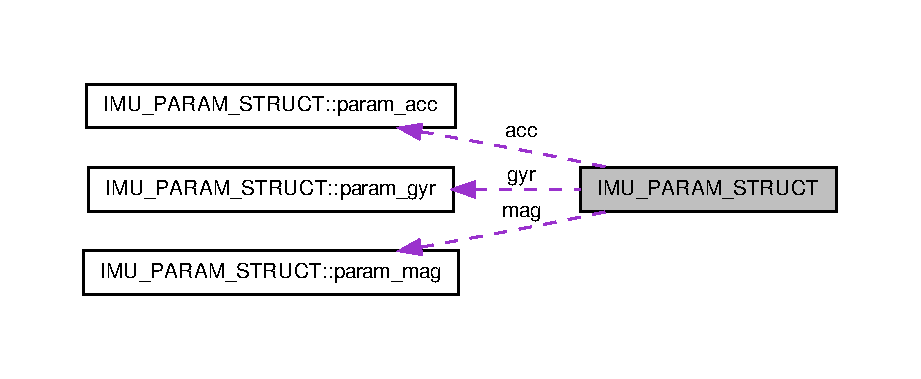
\includegraphics[width=350pt]{structIMU__PARAM__STRUCT__coll__graph}
\end{center}
\end{figure}
\subsection*{Data Structures}
\begin{DoxyCompactItemize}
\item 
struct \hyperlink{structIMU__PARAM__STRUCT_1_1param__acc}{param\-\_\-acc}
\begin{DoxyCompactList}\small\item\em Accelerometer Parameters. \end{DoxyCompactList}\item 
struct \hyperlink{structIMU__PARAM__STRUCT_1_1param__gyr}{param\-\_\-gyr}
\begin{DoxyCompactList}\small\item\em Gyrometer Parameters. \end{DoxyCompactList}\item 
struct \hyperlink{structIMU__PARAM__STRUCT_1_1param__mag}{param\-\_\-mag}
\begin{DoxyCompactList}\small\item\em Magnetometer Parameters. \end{DoxyCompactList}\end{DoxyCompactItemize}
\subsection*{Data Fields}
\begin{DoxyCompactItemize}
\item 
struct \hyperlink{structIMU__PARAM__STRUCT_1_1param__acc}{I\-M\-U\-\_\-\-P\-A\-R\-A\-M\-\_\-\-S\-T\-R\-U\-C\-T\-::param\-\_\-acc} \hyperlink{structIMU__PARAM__STRUCT_a92172e4757d0f8f9135a659e406c12e5}{acc}
\item 
struct \hyperlink{structIMU__PARAM__STRUCT_1_1param__gyr}{I\-M\-U\-\_\-\-P\-A\-R\-A\-M\-\_\-\-S\-T\-R\-U\-C\-T\-::param\-\_\-gyr} \hyperlink{structIMU__PARAM__STRUCT_a5a4557868f1af679a1098808397b02ec}{gyr}
\item 
struct \hyperlink{structIMU__PARAM__STRUCT_1_1param__mag}{I\-M\-U\-\_\-\-P\-A\-R\-A\-M\-\_\-\-S\-T\-R\-U\-C\-T\-::param\-\_\-mag} \hyperlink{structIMU__PARAM__STRUCT_a26b277dcaf05f3842995df888225f6f4}{mag}
\item 
int \hyperlink{structIMU__PARAM__STRUCT_a8a870f383fc9ba0b682fdc9b8c0d2734}{i2c\-\_\-dev}
\end{DoxyCompactItemize}


\subsection{Detailed Description}
Configs of I\-M\-U. 

Definition at line 31 of file communication.\-h.



\subsection{Field Documentation}
\hypertarget{structIMU__PARAM__STRUCT_a92172e4757d0f8f9135a659e406c12e5}{\index{I\-M\-U\-\_\-\-P\-A\-R\-A\-M\-\_\-\-S\-T\-R\-U\-C\-T@{I\-M\-U\-\_\-\-P\-A\-R\-A\-M\-\_\-\-S\-T\-R\-U\-C\-T}!acc@{acc}}
\index{acc@{acc}!IMU_PARAM_STRUCT@{I\-M\-U\-\_\-\-P\-A\-R\-A\-M\-\_\-\-S\-T\-R\-U\-C\-T}}
\subsubsection[{acc}]{\setlength{\rightskip}{0pt plus 5cm}struct {\bf I\-M\-U\-\_\-\-P\-A\-R\-A\-M\-\_\-\-S\-T\-R\-U\-C\-T\-::param\-\_\-acc} I\-M\-U\-\_\-\-P\-A\-R\-A\-M\-\_\-\-S\-T\-R\-U\-C\-T\-::acc}}\label{structIMU__PARAM__STRUCT_a92172e4757d0f8f9135a659e406c12e5}


Referenced by devices\-\_\-init(), and main().

\hypertarget{structIMU__PARAM__STRUCT_a5a4557868f1af679a1098808397b02ec}{\index{I\-M\-U\-\_\-\-P\-A\-R\-A\-M\-\_\-\-S\-T\-R\-U\-C\-T@{I\-M\-U\-\_\-\-P\-A\-R\-A\-M\-\_\-\-S\-T\-R\-U\-C\-T}!gyr@{gyr}}
\index{gyr@{gyr}!IMU_PARAM_STRUCT@{I\-M\-U\-\_\-\-P\-A\-R\-A\-M\-\_\-\-S\-T\-R\-U\-C\-T}}
\subsubsection[{gyr}]{\setlength{\rightskip}{0pt plus 5cm}struct {\bf I\-M\-U\-\_\-\-P\-A\-R\-A\-M\-\_\-\-S\-T\-R\-U\-C\-T\-::param\-\_\-gyr} I\-M\-U\-\_\-\-P\-A\-R\-A\-M\-\_\-\-S\-T\-R\-U\-C\-T\-::gyr}}\label{structIMU__PARAM__STRUCT_a5a4557868f1af679a1098808397b02ec}


Referenced by devices\-\_\-init(), and main().

\hypertarget{structIMU__PARAM__STRUCT_a8a870f383fc9ba0b682fdc9b8c0d2734}{\index{I\-M\-U\-\_\-\-P\-A\-R\-A\-M\-\_\-\-S\-T\-R\-U\-C\-T@{I\-M\-U\-\_\-\-P\-A\-R\-A\-M\-\_\-\-S\-T\-R\-U\-C\-T}!i2c\-\_\-dev@{i2c\-\_\-dev}}
\index{i2c\-\_\-dev@{i2c\-\_\-dev}!IMU_PARAM_STRUCT@{I\-M\-U\-\_\-\-P\-A\-R\-A\-M\-\_\-\-S\-T\-R\-U\-C\-T}}
\subsubsection[{i2c\-\_\-dev}]{\setlength{\rightskip}{0pt plus 5cm}int I\-M\-U\-\_\-\-P\-A\-R\-A\-M\-\_\-\-S\-T\-R\-U\-C\-T\-::i2c\-\_\-dev}}\label{structIMU__PARAM__STRUCT_a8a870f383fc9ba0b682fdc9b8c0d2734}


Definition at line 59 of file communication.\-h.



Referenced by devices\-\_\-init(), main(), periodic\-\_\-task\-\_\-1(), and periodic\-\_\-task\-\_\-2().

\hypertarget{structIMU__PARAM__STRUCT_a26b277dcaf05f3842995df888225f6f4}{\index{I\-M\-U\-\_\-\-P\-A\-R\-A\-M\-\_\-\-S\-T\-R\-U\-C\-T@{I\-M\-U\-\_\-\-P\-A\-R\-A\-M\-\_\-\-S\-T\-R\-U\-C\-T}!mag@{mag}}
\index{mag@{mag}!IMU_PARAM_STRUCT@{I\-M\-U\-\_\-\-P\-A\-R\-A\-M\-\_\-\-S\-T\-R\-U\-C\-T}}
\subsubsection[{mag}]{\setlength{\rightskip}{0pt plus 5cm}struct {\bf I\-M\-U\-\_\-\-P\-A\-R\-A\-M\-\_\-\-S\-T\-R\-U\-C\-T\-::param\-\_\-mag} I\-M\-U\-\_\-\-P\-A\-R\-A\-M\-\_\-\-S\-T\-R\-U\-C\-T\-::mag}}\label{structIMU__PARAM__STRUCT_a26b277dcaf05f3842995df888225f6f4}


Referenced by main().



The documentation for this struct was generated from the following file\-:\begin{DoxyCompactItemize}
\item 
communication/\hyperlink{communication_2communication_8h}{communication.\-h}\end{DoxyCompactItemize}

\hypertarget{structMRA__DATA__STRUCT}{\section{M\-R\-A\-\_\-\-D\-A\-T\-A\-\_\-\-S\-T\-R\-U\-C\-T Struct Reference}
\label{structMRA__DATA__STRUCT}\index{M\-R\-A\-\_\-\-D\-A\-T\-A\-\_\-\-S\-T\-R\-U\-C\-T@{M\-R\-A\-\_\-\-D\-A\-T\-A\-\_\-\-S\-T\-R\-U\-C\-T}}
}


Struct to control M\-R\-A.  




{\ttfamily \#include \char`\"{}communication.\-h\char`\"{}}

\subsection*{Data Fields}
\begin{DoxyCompactItemize}
\item 
short int \hyperlink{structMRA__DATA__STRUCT_a64b4e6bb604e58de593a60c87942b966}{v\-\_\-ctl}
\begin{DoxyCompactList}\small\item\em Voltage level for control output. \end{DoxyCompactList}\item 
short int \hyperlink{structMRA__DATA__STRUCT_a3a31d57268c33b21ac915fdc27dfe474}{v\-\_\-ctl\-\_\-read}
\begin{DoxyCompactList}\small\item\em Voltage level read from the actuator. \end{DoxyCompactList}\item 
int \hyperlink{structMRA__DATA__STRUCT_afca6e851d302f3a786885a4e1eec79d7}{new\-\_\-data}
\begin{DoxyCompactList}\small\item\em ?? \end{DoxyCompactList}\item 
int \hyperlink{structMRA__DATA__STRUCT_a5b1af89ee717f5b14c18e8ac12e93e75}{new\-\_\-ctl}
\begin{DoxyCompactList}\small\item\em ?? \end{DoxyCompactList}\end{DoxyCompactItemize}


\subsection{Detailed Description}
Struct to control M\-R\-A. 

Definition at line 126 of file communication.\-h.



\subsection{Field Documentation}
\hypertarget{structMRA__DATA__STRUCT_a5b1af89ee717f5b14c18e8ac12e93e75}{\index{M\-R\-A\-\_\-\-D\-A\-T\-A\-\_\-\-S\-T\-R\-U\-C\-T@{M\-R\-A\-\_\-\-D\-A\-T\-A\-\_\-\-S\-T\-R\-U\-C\-T}!new\-\_\-ctl@{new\-\_\-ctl}}
\index{new\-\_\-ctl@{new\-\_\-ctl}!MRA_DATA_STRUCT@{M\-R\-A\-\_\-\-D\-A\-T\-A\-\_\-\-S\-T\-R\-U\-C\-T}}
\subsubsection[{new\-\_\-ctl}]{\setlength{\rightskip}{0pt plus 5cm}int M\-R\-A\-\_\-\-D\-A\-T\-A\-\_\-\-S\-T\-R\-U\-C\-T\-::new\-\_\-ctl}}\label{structMRA__DATA__STRUCT_a5b1af89ee717f5b14c18e8ac12e93e75}


?? 



Definition at line 130 of file communication.\-h.



Referenced by actuate(), and devices\-\_\-init().

\hypertarget{structMRA__DATA__STRUCT_afca6e851d302f3a786885a4e1eec79d7}{\index{M\-R\-A\-\_\-\-D\-A\-T\-A\-\_\-\-S\-T\-R\-U\-C\-T@{M\-R\-A\-\_\-\-D\-A\-T\-A\-\_\-\-S\-T\-R\-U\-C\-T}!new\-\_\-data@{new\-\_\-data}}
\index{new\-\_\-data@{new\-\_\-data}!MRA_DATA_STRUCT@{M\-R\-A\-\_\-\-D\-A\-T\-A\-\_\-\-S\-T\-R\-U\-C\-T}}
\subsubsection[{new\-\_\-data}]{\setlength{\rightskip}{0pt plus 5cm}int M\-R\-A\-\_\-\-D\-A\-T\-A\-\_\-\-S\-T\-R\-U\-C\-T\-::new\-\_\-data}}\label{structMRA__DATA__STRUCT_afca6e851d302f3a786885a4e1eec79d7}


?? 



Definition at line 129 of file communication.\-h.



Referenced by read\-\_\-all\-\_\-data().

\hypertarget{structMRA__DATA__STRUCT_a64b4e6bb604e58de593a60c87942b966}{\index{M\-R\-A\-\_\-\-D\-A\-T\-A\-\_\-\-S\-T\-R\-U\-C\-T@{M\-R\-A\-\_\-\-D\-A\-T\-A\-\_\-\-S\-T\-R\-U\-C\-T}!v\-\_\-ctl@{v\-\_\-ctl}}
\index{v\-\_\-ctl@{v\-\_\-ctl}!MRA_DATA_STRUCT@{M\-R\-A\-\_\-\-D\-A\-T\-A\-\_\-\-S\-T\-R\-U\-C\-T}}
\subsubsection[{v\-\_\-ctl}]{\setlength{\rightskip}{0pt plus 5cm}short int M\-R\-A\-\_\-\-D\-A\-T\-A\-\_\-\-S\-T\-R\-U\-C\-T\-::v\-\_\-ctl}}\label{structMRA__DATA__STRUCT_a64b4e6bb604e58de593a60c87942b966}


Voltage level for control output. 



Definition at line 127 of file communication.\-h.



Referenced by actuate(), control\-\_\-main(), datalogger\-\_\-update(), devices\-\_\-init(), periodic\-\_\-task\-\_\-1(), ui\-\_\-mra\-\_\-data(), and ui\-\_\-overview\-\_\-data().

\hypertarget{structMRA__DATA__STRUCT_a3a31d57268c33b21ac915fdc27dfe474}{\index{M\-R\-A\-\_\-\-D\-A\-T\-A\-\_\-\-S\-T\-R\-U\-C\-T@{M\-R\-A\-\_\-\-D\-A\-T\-A\-\_\-\-S\-T\-R\-U\-C\-T}!v\-\_\-ctl\-\_\-read@{v\-\_\-ctl\-\_\-read}}
\index{v\-\_\-ctl\-\_\-read@{v\-\_\-ctl\-\_\-read}!MRA_DATA_STRUCT@{M\-R\-A\-\_\-\-D\-A\-T\-A\-\_\-\-S\-T\-R\-U\-C\-T}}
\subsubsection[{v\-\_\-ctl\-\_\-read}]{\setlength{\rightskip}{0pt plus 5cm}short int M\-R\-A\-\_\-\-D\-A\-T\-A\-\_\-\-S\-T\-R\-U\-C\-T\-::v\-\_\-ctl\-\_\-read}}\label{structMRA__DATA__STRUCT_a3a31d57268c33b21ac915fdc27dfe474}


Voltage level read from the actuator. 



Definition at line 128 of file communication.\-h.



Referenced by datalogger\-\_\-update(), read\-\_\-all\-\_\-data(), ui\-\_\-mra\-\_\-data(), and ui\-\_\-overview\-\_\-data().



The documentation for this struct was generated from the following file\-:\begin{DoxyCompactItemize}
\item 
communication/\hyperlink{communication_2communication_8h}{communication.\-h}\end{DoxyCompactItemize}

\hypertarget{structIMU__PARAM__STRUCT_1_1param__acc}{\section{I\-M\-U\-\_\-\-P\-A\-R\-A\-M\-\_\-\-S\-T\-R\-U\-C\-T\-:\-:param\-\_\-acc Struct Reference}
\label{structIMU__PARAM__STRUCT_1_1param__acc}\index{I\-M\-U\-\_\-\-P\-A\-R\-A\-M\-\_\-\-S\-T\-R\-U\-C\-T\-::param\-\_\-acc@{I\-M\-U\-\_\-\-P\-A\-R\-A\-M\-\_\-\-S\-T\-R\-U\-C\-T\-::param\-\_\-acc}}
}


Accelerometer Parameters.  




{\ttfamily \#include \char`\"{}communication.\-h\char`\"{}}

\subsection*{Data Fields}
\begin{DoxyCompactItemize}
\item 
uint8\-\_\-t \hyperlink{structIMU__PARAM__STRUCT_1_1param__acc_af57da5d956ffa7e49a184326b6b9c738}{full\-\_\-res}
\item 
uint16\-\_\-t \hyperlink{structIMU__PARAM__STRUCT_1_1param__acc_a30e6a318cad098cd8379416705820f95}{rate}
\item 
uint8\-\_\-t \hyperlink{structIMU__PARAM__STRUCT_1_1param__acc_a26199b298ef2d353192dfbc706bce8cf}{range}
\end{DoxyCompactItemize}


\subsection{Detailed Description}
Accelerometer Parameters. 

Definition at line 35 of file communication.\-h.



\subsection{Field Documentation}
\hypertarget{structIMU__PARAM__STRUCT_1_1param__acc_af57da5d956ffa7e49a184326b6b9c738}{\index{I\-M\-U\-\_\-\-P\-A\-R\-A\-M\-\_\-\-S\-T\-R\-U\-C\-T\-::param\-\_\-acc@{I\-M\-U\-\_\-\-P\-A\-R\-A\-M\-\_\-\-S\-T\-R\-U\-C\-T\-::param\-\_\-acc}!full\-\_\-res@{full\-\_\-res}}
\index{full\-\_\-res@{full\-\_\-res}!IMU_PARAM_STRUCT::param_acc@{I\-M\-U\-\_\-\-P\-A\-R\-A\-M\-\_\-\-S\-T\-R\-U\-C\-T\-::param\-\_\-acc}}
\subsubsection[{full\-\_\-res}]{\setlength{\rightskip}{0pt plus 5cm}uint8\-\_\-t I\-M\-U\-\_\-\-P\-A\-R\-A\-M\-\_\-\-S\-T\-R\-U\-C\-T\-::param\-\_\-acc\-::full\-\_\-res}}\label{structIMU__PARAM__STRUCT_1_1param__acc_af57da5d956ffa7e49a184326b6b9c738}


Definition at line 36 of file communication.\-h.



Referenced by devices\-\_\-init(), and main().

\hypertarget{structIMU__PARAM__STRUCT_1_1param__acc_a26199b298ef2d353192dfbc706bce8cf}{\index{I\-M\-U\-\_\-\-P\-A\-R\-A\-M\-\_\-\-S\-T\-R\-U\-C\-T\-::param\-\_\-acc@{I\-M\-U\-\_\-\-P\-A\-R\-A\-M\-\_\-\-S\-T\-R\-U\-C\-T\-::param\-\_\-acc}!range@{range}}
\index{range@{range}!IMU_PARAM_STRUCT::param_acc@{I\-M\-U\-\_\-\-P\-A\-R\-A\-M\-\_\-\-S\-T\-R\-U\-C\-T\-::param\-\_\-acc}}
\subsubsection[{range}]{\setlength{\rightskip}{0pt plus 5cm}uint8\-\_\-t I\-M\-U\-\_\-\-P\-A\-R\-A\-M\-\_\-\-S\-T\-R\-U\-C\-T\-::param\-\_\-acc\-::range}}\label{structIMU__PARAM__STRUCT_1_1param__acc_a26199b298ef2d353192dfbc706bce8cf}


Definition at line 38 of file communication.\-h.



Referenced by devices\-\_\-init(), and main().

\hypertarget{structIMU__PARAM__STRUCT_1_1param__acc_a30e6a318cad098cd8379416705820f95}{\index{I\-M\-U\-\_\-\-P\-A\-R\-A\-M\-\_\-\-S\-T\-R\-U\-C\-T\-::param\-\_\-acc@{I\-M\-U\-\_\-\-P\-A\-R\-A\-M\-\_\-\-S\-T\-R\-U\-C\-T\-::param\-\_\-acc}!rate@{rate}}
\index{rate@{rate}!IMU_PARAM_STRUCT::param_acc@{I\-M\-U\-\_\-\-P\-A\-R\-A\-M\-\_\-\-S\-T\-R\-U\-C\-T\-::param\-\_\-acc}}
\subsubsection[{rate}]{\setlength{\rightskip}{0pt plus 5cm}uint16\-\_\-t I\-M\-U\-\_\-\-P\-A\-R\-A\-M\-\_\-\-S\-T\-R\-U\-C\-T\-::param\-\_\-acc\-::rate}}\label{structIMU__PARAM__STRUCT_1_1param__acc_a30e6a318cad098cd8379416705820f95}


Definition at line 37 of file communication.\-h.



Referenced by devices\-\_\-init(), and main().



The documentation for this struct was generated from the following file\-:\begin{DoxyCompactItemize}
\item 
communication/\hyperlink{communication_2communication_8h}{communication.\-h}\end{DoxyCompactItemize}

\hypertarget{structIMU__PARAM__STRUCT_1_1param__gyr}{\section{I\-M\-U\-\_\-\-P\-A\-R\-A\-M\-\_\-\-S\-T\-R\-U\-C\-T\-:\-:param\-\_\-gyr Struct Reference}
\label{structIMU__PARAM__STRUCT_1_1param__gyr}\index{I\-M\-U\-\_\-\-P\-A\-R\-A\-M\-\_\-\-S\-T\-R\-U\-C\-T\-::param\-\_\-gyr@{I\-M\-U\-\_\-\-P\-A\-R\-A\-M\-\_\-\-S\-T\-R\-U\-C\-T\-::param\-\_\-gyr}}
}


Gyrometer Parameters.  




{\ttfamily \#include \char`\"{}communication.\-h\char`\"{}}

\subsection*{Data Fields}
\begin{DoxyCompactItemize}
\item 
float \hyperlink{structIMU__PARAM__STRUCT_1_1param__gyr_a5aa70e1e9634411c89aacfbc570cc91c}{rate}
\item 
short int \hyperlink{structIMU__PARAM__STRUCT_1_1param__gyr_aa612f7299b43a1bf1fc597688c2fa02d}{lpf\-\_\-bw}
\item 
char \hyperlink{structIMU__PARAM__STRUCT_1_1param__gyr_aca3b791cb480f2da4703d4c256a7de48}{clk\-\_\-source}
\item 
char $\ast$ \hyperlink{structIMU__PARAM__STRUCT_1_1param__gyr_a909d153e794ec443be04625ce00e4178}{act}
\end{DoxyCompactItemize}


\subsection{Detailed Description}
Gyrometer Parameters. 

Definition at line 43 of file communication.\-h.



\subsection{Field Documentation}
\hypertarget{structIMU__PARAM__STRUCT_1_1param__gyr_a909d153e794ec443be04625ce00e4178}{\index{I\-M\-U\-\_\-\-P\-A\-R\-A\-M\-\_\-\-S\-T\-R\-U\-C\-T\-::param\-\_\-gyr@{I\-M\-U\-\_\-\-P\-A\-R\-A\-M\-\_\-\-S\-T\-R\-U\-C\-T\-::param\-\_\-gyr}!act@{act}}
\index{act@{act}!IMU_PARAM_STRUCT::param_gyr@{I\-M\-U\-\_\-\-P\-A\-R\-A\-M\-\_\-\-S\-T\-R\-U\-C\-T\-::param\-\_\-gyr}}
\subsubsection[{act}]{\setlength{\rightskip}{0pt plus 5cm}char$\ast$ I\-M\-U\-\_\-\-P\-A\-R\-A\-M\-\_\-\-S\-T\-R\-U\-C\-T\-::param\-\_\-gyr\-::act}}\label{structIMU__PARAM__STRUCT_1_1param__gyr_a909d153e794ec443be04625ce00e4178}


Definition at line 47 of file communication.\-h.



Referenced by devices\-\_\-init(), and main().

\hypertarget{structIMU__PARAM__STRUCT_1_1param__gyr_aca3b791cb480f2da4703d4c256a7de48}{\index{I\-M\-U\-\_\-\-P\-A\-R\-A\-M\-\_\-\-S\-T\-R\-U\-C\-T\-::param\-\_\-gyr@{I\-M\-U\-\_\-\-P\-A\-R\-A\-M\-\_\-\-S\-T\-R\-U\-C\-T\-::param\-\_\-gyr}!clk\-\_\-source@{clk\-\_\-source}}
\index{clk\-\_\-source@{clk\-\_\-source}!IMU_PARAM_STRUCT::param_gyr@{I\-M\-U\-\_\-\-P\-A\-R\-A\-M\-\_\-\-S\-T\-R\-U\-C\-T\-::param\-\_\-gyr}}
\subsubsection[{clk\-\_\-source}]{\setlength{\rightskip}{0pt plus 5cm}char I\-M\-U\-\_\-\-P\-A\-R\-A\-M\-\_\-\-S\-T\-R\-U\-C\-T\-::param\-\_\-gyr\-::clk\-\_\-source}}\label{structIMU__PARAM__STRUCT_1_1param__gyr_aca3b791cb480f2da4703d4c256a7de48}


Definition at line 46 of file communication.\-h.



Referenced by devices\-\_\-init(), and main().

\hypertarget{structIMU__PARAM__STRUCT_1_1param__gyr_aa612f7299b43a1bf1fc597688c2fa02d}{\index{I\-M\-U\-\_\-\-P\-A\-R\-A\-M\-\_\-\-S\-T\-R\-U\-C\-T\-::param\-\_\-gyr@{I\-M\-U\-\_\-\-P\-A\-R\-A\-M\-\_\-\-S\-T\-R\-U\-C\-T\-::param\-\_\-gyr}!lpf\-\_\-bw@{lpf\-\_\-bw}}
\index{lpf\-\_\-bw@{lpf\-\_\-bw}!IMU_PARAM_STRUCT::param_gyr@{I\-M\-U\-\_\-\-P\-A\-R\-A\-M\-\_\-\-S\-T\-R\-U\-C\-T\-::param\-\_\-gyr}}
\subsubsection[{lpf\-\_\-bw}]{\setlength{\rightskip}{0pt plus 5cm}short int I\-M\-U\-\_\-\-P\-A\-R\-A\-M\-\_\-\-S\-T\-R\-U\-C\-T\-::param\-\_\-gyr\-::lpf\-\_\-bw}}\label{structIMU__PARAM__STRUCT_1_1param__gyr_aa612f7299b43a1bf1fc597688c2fa02d}


Definition at line 45 of file communication.\-h.



Referenced by devices\-\_\-init(), and main().

\hypertarget{structIMU__PARAM__STRUCT_1_1param__gyr_a5aa70e1e9634411c89aacfbc570cc91c}{\index{I\-M\-U\-\_\-\-P\-A\-R\-A\-M\-\_\-\-S\-T\-R\-U\-C\-T\-::param\-\_\-gyr@{I\-M\-U\-\_\-\-P\-A\-R\-A\-M\-\_\-\-S\-T\-R\-U\-C\-T\-::param\-\_\-gyr}!rate@{rate}}
\index{rate@{rate}!IMU_PARAM_STRUCT::param_gyr@{I\-M\-U\-\_\-\-P\-A\-R\-A\-M\-\_\-\-S\-T\-R\-U\-C\-T\-::param\-\_\-gyr}}
\subsubsection[{rate}]{\setlength{\rightskip}{0pt plus 5cm}float I\-M\-U\-\_\-\-P\-A\-R\-A\-M\-\_\-\-S\-T\-R\-U\-C\-T\-::param\-\_\-gyr\-::rate}}\label{structIMU__PARAM__STRUCT_1_1param__gyr_a5aa70e1e9634411c89aacfbc570cc91c}


Definition at line 44 of file communication.\-h.



Referenced by devices\-\_\-init(), and main().



The documentation for this struct was generated from the following file\-:\begin{DoxyCompactItemize}
\item 
communication/\hyperlink{communication_2communication_8h}{communication.\-h}\end{DoxyCompactItemize}

\hypertarget{structIMU__PARAM__STRUCT_1_1param__mag}{
\section{IMU\_\-PARAM\_\-STRUCT::param\_\-mag Struct Reference}
\label{structIMU__PARAM__STRUCT_1_1param__mag}\index{IMU\_\-PARAM\_\-STRUCT::param\_\-mag@{IMU\_\-PARAM\_\-STRUCT::param\_\-mag}}
}
\subsection*{Data Fields}
\begin{DoxyCompactItemize}
\item 
\hypertarget{structIMU__PARAM__STRUCT_1_1param__mag_a234de95423b604b05b851ef90890cea1}{
uint8\_\-t {\bfseries rate}}
\label{structIMU__PARAM__STRUCT_1_1param__mag_a234de95423b604b05b851ef90890cea1}

\item 
\hypertarget{structIMU__PARAM__STRUCT_1_1param__mag_a40ad27ebdb5fde35257b1dc52e40f476}{
uint8\_\-t {\bfseries range}}
\label{structIMU__PARAM__STRUCT_1_1param__mag_a40ad27ebdb5fde35257b1dc52e40f476}

\item 
\hypertarget{structIMU__PARAM__STRUCT_1_1param__mag_a52c22cae6940eb39fb72aca66cfeba9a}{
uint8\_\-t {\bfseries samples\_\-avg}}
\label{structIMU__PARAM__STRUCT_1_1param__mag_a52c22cae6940eb39fb72aca66cfeba9a}

\item 
\hypertarget{structIMU__PARAM__STRUCT_1_1param__mag_a1f3536709c05310005d648f339d70c54}{
uint8\_\-t {\bfseries meas\_\-mode}}
\label{structIMU__PARAM__STRUCT_1_1param__mag_a1f3536709c05310005d648f339d70c54}

\item 
\hypertarget{structIMU__PARAM__STRUCT_1_1param__mag_a39b83b3e9ff5bdcafed0bdf6a2de584b}{
uint8\_\-t {\bfseries op\_\-mode}}
\label{structIMU__PARAM__STRUCT_1_1param__mag_a39b83b3e9ff5bdcafed0bdf6a2de584b}

\end{DoxyCompactItemize}


The documentation for this struct was generated from the following files:\begin{DoxyCompactItemize}
\item 
communication/communication (Cópia em conflito de Caio Gustavo Mesquita Angelo 2013-\/05-\/17).h\item 
communication/communication.h\end{DoxyCompactItemize}

\hypertarget{structSPI__PARAM__STRUCT}{\section{S\-P\-I\-\_\-\-P\-A\-R\-A\-M\-\_\-\-S\-T\-R\-U\-C\-T Struct Reference}
\label{structSPI__PARAM__STRUCT}\index{S\-P\-I\-\_\-\-P\-A\-R\-A\-M\-\_\-\-S\-T\-R\-U\-C\-T@{S\-P\-I\-\_\-\-P\-A\-R\-A\-M\-\_\-\-S\-T\-R\-U\-C\-T}}
}


Configs for S\-P\-I.  




{\ttfamily \#include \char`\"{}communication.\-h\char`\"{}}

\subsection*{Data Fields}
\begin{DoxyCompactItemize}
\item 
uint8\-\_\-t \hyperlink{structSPI__PARAM__STRUCT_a82c546c99f6c3daed73c1e23426be847}{mode}
\item 
uint32\-\_\-t \hyperlink{structSPI__PARAM__STRUCT_a53a8d386594a81eb9bc6f971bfe36c54}{speed}
\item 
uint8\-\_\-t \hyperlink{structSPI__PARAM__STRUCT_ae0d62e0a5554783d710b677a017e246f}{cs}
\item 
int \hyperlink{structSPI__PARAM__STRUCT_abe385c44333d268d17cf648c8e371cad}{spi\-\_\-dev}
\end{DoxyCompactItemize}


\subsection{Detailed Description}
Configs for S\-P\-I. 

Definition at line 65 of file communication.\-h.



\subsection{Field Documentation}
\hypertarget{structSPI__PARAM__STRUCT_ae0d62e0a5554783d710b677a017e246f}{\index{S\-P\-I\-\_\-\-P\-A\-R\-A\-M\-\_\-\-S\-T\-R\-U\-C\-T@{S\-P\-I\-\_\-\-P\-A\-R\-A\-M\-\_\-\-S\-T\-R\-U\-C\-T}!cs@{cs}}
\index{cs@{cs}!SPI_PARAM_STRUCT@{S\-P\-I\-\_\-\-P\-A\-R\-A\-M\-\_\-\-S\-T\-R\-U\-C\-T}}
\subsubsection[{cs}]{\setlength{\rightskip}{0pt plus 5cm}uint8\-\_\-t S\-P\-I\-\_\-\-P\-A\-R\-A\-M\-\_\-\-S\-T\-R\-U\-C\-T\-::cs}}\label{structSPI__PARAM__STRUCT_ae0d62e0a5554783d710b677a017e246f}


Definition at line 68 of file communication.\-h.



Referenced by devices\-\_\-init(), and main().

\hypertarget{structSPI__PARAM__STRUCT_a82c546c99f6c3daed73c1e23426be847}{\index{S\-P\-I\-\_\-\-P\-A\-R\-A\-M\-\_\-\-S\-T\-R\-U\-C\-T@{S\-P\-I\-\_\-\-P\-A\-R\-A\-M\-\_\-\-S\-T\-R\-U\-C\-T}!mode@{mode}}
\index{mode@{mode}!SPI_PARAM_STRUCT@{S\-P\-I\-\_\-\-P\-A\-R\-A\-M\-\_\-\-S\-T\-R\-U\-C\-T}}
\subsubsection[{mode}]{\setlength{\rightskip}{0pt plus 5cm}uint8\-\_\-t S\-P\-I\-\_\-\-P\-A\-R\-A\-M\-\_\-\-S\-T\-R\-U\-C\-T\-::mode}}\label{structSPI__PARAM__STRUCT_a82c546c99f6c3daed73c1e23426be847}


Definition at line 66 of file communication.\-h.



Referenced by devices\-\_\-init(), and main().

\hypertarget{structSPI__PARAM__STRUCT_a53a8d386594a81eb9bc6f971bfe36c54}{\index{S\-P\-I\-\_\-\-P\-A\-R\-A\-M\-\_\-\-S\-T\-R\-U\-C\-T@{S\-P\-I\-\_\-\-P\-A\-R\-A\-M\-\_\-\-S\-T\-R\-U\-C\-T}!speed@{speed}}
\index{speed@{speed}!SPI_PARAM_STRUCT@{S\-P\-I\-\_\-\-P\-A\-R\-A\-M\-\_\-\-S\-T\-R\-U\-C\-T}}
\subsubsection[{speed}]{\setlength{\rightskip}{0pt plus 5cm}uint32\-\_\-t S\-P\-I\-\_\-\-P\-A\-R\-A\-M\-\_\-\-S\-T\-R\-U\-C\-T\-::speed}}\label{structSPI__PARAM__STRUCT_a53a8d386594a81eb9bc6f971bfe36c54}


Definition at line 67 of file communication.\-h.



Referenced by devices\-\_\-init(), and main().

\hypertarget{structSPI__PARAM__STRUCT_abe385c44333d268d17cf648c8e371cad}{\index{S\-P\-I\-\_\-\-P\-A\-R\-A\-M\-\_\-\-S\-T\-R\-U\-C\-T@{S\-P\-I\-\_\-\-P\-A\-R\-A\-M\-\_\-\-S\-T\-R\-U\-C\-T}!spi\-\_\-dev@{spi\-\_\-dev}}
\index{spi\-\_\-dev@{spi\-\_\-dev}!SPI_PARAM_STRUCT@{S\-P\-I\-\_\-\-P\-A\-R\-A\-M\-\_\-\-S\-T\-R\-U\-C\-T}}
\subsubsection[{spi\-\_\-dev}]{\setlength{\rightskip}{0pt plus 5cm}int S\-P\-I\-\_\-\-P\-A\-R\-A\-M\-\_\-\-S\-T\-R\-U\-C\-T\-::spi\-\_\-dev}}\label{structSPI__PARAM__STRUCT_abe385c44333d268d17cf648c8e371cad}


Definition at line 69 of file communication.\-h.



Referenced by devices\-\_\-init(), main(), periodic\-\_\-task\-\_\-1(), and periodic\-\_\-task\-\_\-2().



The documentation for this struct was generated from the following file\-:\begin{DoxyCompactItemize}
\item 
communication/\hyperlink{communication_2communication_8h}{communication.\-h}\end{DoxyCompactItemize}

\printindex
\end{document}
